% =============================================================================
% Figure 1E-3: Phase accumulator internals (textbook DDS view)
% =============================================================================
% Zoom-in on the phase accumulator that runs in Pico Core 1 firmware. Shows the
% canonical NCO building blocks: FTW register, adder (with chevron notch on the
% input side separating the two summed operands), and the phase register with
% its feedback loop. The phase register is clocked by f_CLK (the same sample
% clock driving the DAC).
%
% Modeled on the Analog Devices DDS Tutorial figure and standard textbook NCO
% diagrams (Frequency Register -> Adder -> Phase Register with feedback).
%
% Compile:  pdflatex 1e_phase_accumulator.tex
% Convert:  pdftocairo -svg 1e_phase_accumulator.pdf
% =============================================================================
\documentclass[border=8pt]{standalone}
%
% =============================================================================
% pmvb-figures.sty -- Poor Man's Validation Bench figure style sheet
% =============================================================================
% Defines the house style for all TikZ figures in PMVB design documents.
%
% Usage in figure source:
%     \documentclass[border=4pt]{standalone}
%     \usepackage{pmvb-figures}
%
% Two color modes:
%     \pmvbDarkMode   -- dark background (default; matches SDD HTML theme)
%     \pmvbLightMode  -- white background (for printed portfolio PDFs)
% =============================================================================
\NeedsTeXFormat{LaTeX2e}
\ProvidesPackage{pmvb-figures}[2026/05/06 PMVB figure styles]
%
% --- Required packages ------------------------------------------------------
\RequirePackage{tikz}
% NOTE: dropped the siunitx option. Our figures use \pmvblabel{} for unit
% annotations rather than circuitikz's SI value formatting, and siunitx.sty
% isn't always available on bare TeX Live installs.
\RequirePackage[american]{circuitikz}
\RequirePackage{xcolor}
\RequirePackage{etoolbox}
%
% --- TikZ libraries ---------------------------------------------------------
\usetikzlibrary{arrows.meta}
\usetikzlibrary{positioning}
\usetikzlibrary{shapes.geometric}
\usetikzlibrary{shapes.misc}
\usetikzlibrary{fit}
\usetikzlibrary{backgrounds}
\usetikzlibrary{calc}
\usetikzlibrary{decorations.pathreplacing}
\usetikzlibrary{patterns}
%
% =============================================================================
% Color palette (FMCW dark theme, matches SDD HTML)
% =============================================================================
\definecolor{pmvbBg}{HTML}{0d1117}
\definecolor{pmvbFg}{HTML}{e6edf3}
\definecolor{pmvbMuted}{HTML}{94a3b8}
\definecolor{pmvbBlue}{HTML}{3b82f6}
\definecolor{pmvbBlueFill}{HTML}{1f2937}
\definecolor{pmvbGreen}{HTML}{10b981}
\definecolor{pmvbGreenFill}{HTML}{1e293b}
\definecolor{pmvbAmber}{HTML}{f59e0b}
\definecolor{pmvbRed}{HTML}{ef4444}
\definecolor{pmvbViolet}{HTML}{a78bfa}
%
\definecolor{pmvbBgLight}{HTML}{ffffff}
\definecolor{pmvbFgLight}{HTML}{0f172a}
\definecolor{pmvbMutedLight}{HTML}{475569}
\definecolor{pmvbBlueFillLight}{HTML}{dbeafe}
\definecolor{pmvbGreenFillLight}{HTML}{d1fae5}
%
% =============================================================================
% Mode selectors
% =============================================================================
\newcommand{\pmvbDarkMode}{%
  \pagecolor{pmvbBg}%
  \color{pmvbFg}%
}
%
\newcommand{\pmvbLightMode}{%
  \colorlet{pmvbBg}{pmvbBgLight}%
  \colorlet{pmvbFg}{pmvbFgLight}%
  \colorlet{pmvbMuted}{pmvbMutedLight}%
  \colorlet{pmvbBlueFill}{pmvbBlueFillLight}%
  \colorlet{pmvbGreenFill}{pmvbGreenFillLight}%
  \pagecolor{pmvbBgLight}%
  \color{pmvbFgLight}%
}
%
\AtBeginDocument{\pmvbDarkMode}
%
% =============================================================================
% Node styles
% -----------------------------------------------------------------------------
% IMPORTANT: each \tikzset{...} block below must be a single argument with NO
% blank lines inside, otherwise \par is inserted and pgfkeys errors out.
% =============================================================================
%
% --- Subsystem (system-level block: a board, a chip, a whole module) ---
\tikzset{
  pmvb subsystem/.style={
    rectangle,
    rounded corners=2pt,
    draw=pmvbBlue,
    line width=0.8pt,
    fill=pmvbBlueFill,
    text=pmvbFg,
    minimum width=28mm,
    minimum height=12mm,
    align=center,
    font=\sffamily\small,
    inner sep=4pt,
  },
}
%
% --- IC / hardware part (functional-level block) ---
\tikzset{
  pmvb ic/.style={
    rectangle,
    rounded corners=1pt,
    draw=pmvbGreen,
    line width=0.6pt,
    fill=pmvbGreenFill,
    text=pmvbFg,
    minimum width=24mm,
    minimum height=10mm,
    align=center,
    font=\sffamily\footnotesize,
    inner sep=3pt,
  },
}
%
% --- Internal block (inside an IC's functional block diagram) ---
\tikzset{
  pmvb internal/.style={
    rectangle,
    draw=pmvbFg,
    line width=0.5pt,
    fill=pmvbBg,
    text=pmvbFg,
    minimum width=18mm,
    minimum height=7mm,
    align=center,
    font=\sffamily\scriptsize,
    inner sep=2pt,
  },
}
%
% --- Pin pad (the box-with-X at IC die boundary in datasheet diagrams) ---
\tikzset{
  pmvb pin/.style={
    rectangle,
    draw=pmvbFg,
    line width=0.4pt,
    fill=pmvbBg,
    minimum size=2.5mm,
    inner sep=0pt,
    path picture={
      \draw[pmvbFg, line width=0.3pt]
        (path picture bounding box.south west) -- (path picture bounding box.north east)
        (path picture bounding box.north west) -- (path picture bounding box.south east);
    },
  },
}
%
% --- Connector (front panel, BNC, banana jack) ---
\tikzset{
  pmvb connector/.style={
    circle,
    draw=pmvbFg,
    line width=0.6pt,
    fill=pmvbBg,
    text=pmvbFg,
    minimum size=8mm,
    font=\sffamily\scriptsize,
    inner sep=1pt,
  },
}
%
% --- Annotation (no border, small muted italic text) ---
\tikzset{
  pmvb annotation/.style={
    text=pmvbMuted,
    font=\sffamily\scriptsize\itshape,
    align=center,
  },
}
%
% --- Subsystem grouping box (used with \node[fit=...]) ---
\tikzset{
  pmvb group/.style={
    rectangle,
    rounded corners=4pt,
    draw=pmvbMuted,
    line width=0.4pt,
    dashed,
    text=pmvbMuted,
    inner sep=8pt,
    font=\sffamily\scriptsize,
  },
}
%
% =============================================================================
% Edge styles
% -----------------------------------------------------------------------------
% Edge styles encode the *kind* of signal flowing on the line.
% =============================================================================
%
\tikzset{
  pmvb digital/.style={
    -Stealth,
    draw=pmvbBlue,
    line width=0.8pt,
    font=\sffamily\scriptsize,
  },
}
%
\tikzset{
  pmvb analog/.style={
    -Stealth,
    draw=pmvbAmber,
    line width=0.8pt,
    font=\sffamily\scriptsize,
  },
}
%
\tikzset{
  pmvb power/.style={
    -Stealth,
    draw=pmvbRed,
    line width=1.0pt,
    font=\sffamily\scriptsize,
  },
}
%
\tikzset{
  pmvb control/.style={
    -Stealth,
    draw=pmvbViolet,
    line width=0.7pt,
    dashed,
    font=\sffamily\scriptsize,
  },
}
%
\tikzset{
  pmvb bus/.style={
    -Stealth,
    draw=pmvbBlue,
    line width=1.4pt,
    double=pmvbBg,
    double distance=0.6pt,
    font=\sffamily\scriptsize,
  },
}
%
% Style for the "xN" bus-width annotation (overlaid on a bus line).
% Dark fill masks the underlying double-line so the white text reads cleanly.
\tikzset{
  pmvb bus width/.style={
    fill=pmvbBg,
    rounded corners=1pt,
    inner sep=2pt,
    font=\sffamily\bfseries\scriptsize,
    text=pmvbFg,
  },
}
%
\tikzset{
  pmvb optional/.style={
    -Stealth,
    draw=pmvbMuted,
    line width=0.6pt,
    dashed,
    font=\sffamily\scriptsize,
  },
}
%
% --- Bidirectional variants ---
\tikzset{
  pmvb digital bi/.style={
    pmvb digital,
    Stealth-Stealth,
  },
}
%
\tikzset{
  pmvb analog bi/.style={
    pmvb analog,
    Stealth-Stealth,
  },
}
%
% =============================================================================
% Diagram-level convenience
% =============================================================================
\tikzset{
  pmvb figure/.style={
    >=Stealth,
    every node/.append style={font=\sffamily},
    node distance=10mm and 14mm,
  },
}
%
% =============================================================================
% Helper macros
% =============================================================================
\newcommand{\pmvblabel}[1]{\textcolor{pmvbMuted}{\sffamily\scriptsize\itshape #1}}
%
\newcommand{\pmvbsubsystem}[3]{%
  node[pmvb subsystem] (#1) {{\bfseries #2}\\\scriptsize #3}%
}
%
\newcommand{\pmvbic}[3]{%
  node[pmvb ic] (#1) {{\bfseries #2}\\\scriptsize #3}%
}
%
% NOTE on bus-width annotations: TikZ's path parser doesn't reliably expand
% \newcommand macros at mid-path positions, so for the "xN" overlay use the
% inline node-in-path syntax directly:
%     \draw[pmvb bus] (A) -- node[pmvb bus width]{$\times 16$} (B);
% The pmvb bus width style is defined above.
%
% -----------------------------------------------------------------------------
% \opamptri{name}{coord}{dir}
%   Draws an op-amp triangle. Apex points right (dir=1) or left (dir=-1).
%   Defines coordinates: <name>_p, <name>_n, <name>_out for wiring.
%   Place any label as a separate \node call after the macro.
%
%   The {coord} argument MUST include its own parentheses, e.g.
%       \opamptri{bufa}{(0.6, -0.5)}{1}
%       \opamptri{tl072}{($(m1e.center) + (4mm, -14mm)$)}{1}
%   This lets callers use either simple coords or calc expressions.
% -----------------------------------------------------------------------------
\newcommand{\opamptri}[3]{%
  \begin{scope}[shift={#2}, xscale=#3]
    \draw[pmvbFg, line width=0.6pt, fill=pmvbBg]
      (0, 0) -- (
%
\begin{document}
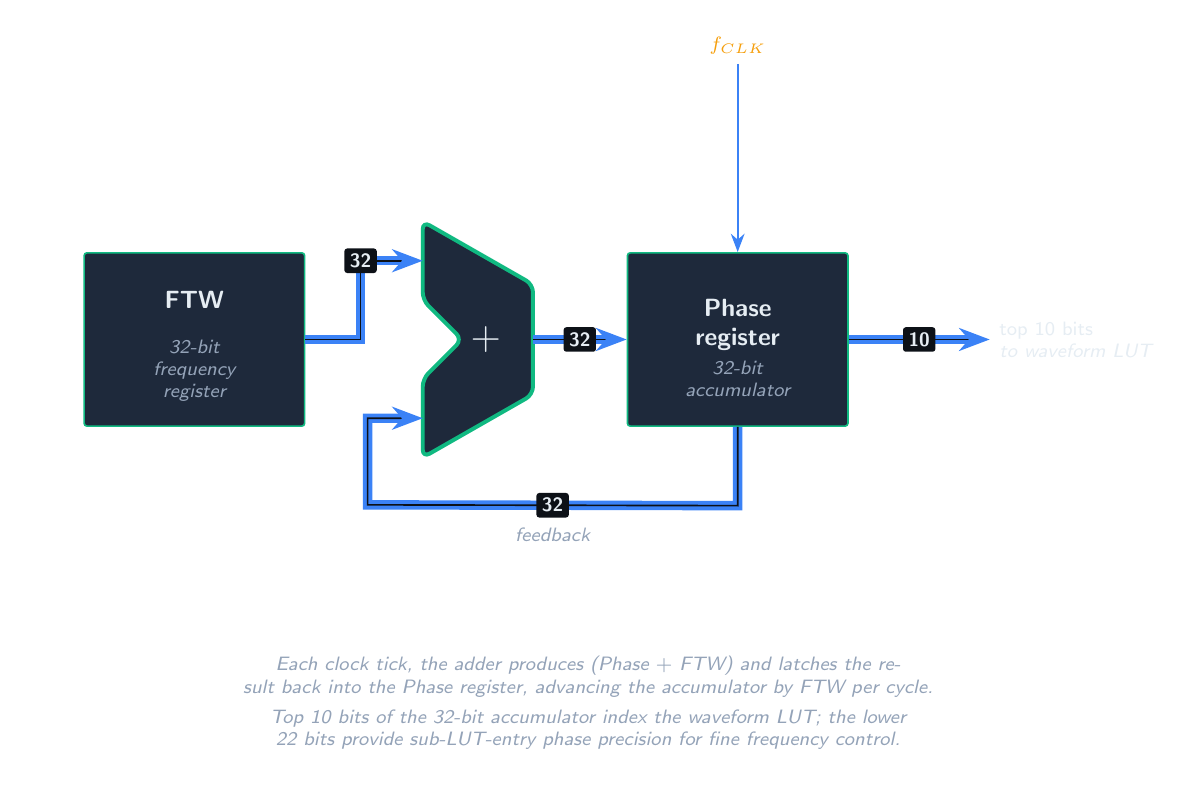
\begin{tikzpicture}[pmvb figure]

  % =========================================================================
  % f_CLK input (directly above phase register, straight vertical arrow)
  % =========================================================================
  \node[font=\sffamily\scriptsize, text=pmvbAmber, anchor=south]
    (fclk) at (8.4, 5.0) {$f_{CLK}$};

  % =========================================================================
  % FTW register on the left
  % =========================================================================
  \node[pmvb ic, minimum width=28mm, minimum height=22mm]
    (ftw) at (1.5, 1.5) {};
  \node[font=\sffamily\bfseries\small, text=pmvbFg, align=center]
    at ([yshift=5mm]ftw.center) {FTW};
  \node[font=\sffamily\scriptsize\itshape, text=pmvbMuted, align=center]
    at ([yshift=-4mm]ftw.center) {32-bit\\frequency\\register};

  % =========================================================================
  % Adder (pentagon with chevron notch on left input side)
  % Clockwise from top-left: top-left -> top-right -> bottom-right ->
  % bottom-left -> notch-bottom -> notch-tip -> notch-top -> cycle.
  % =========================================================================
  \draw[fill=pmvbGreenFill, draw=pmvbGreen, line width=0.5mm, rounded corners=1mm]
    (4.4, 3.0)   % top-left
    -- (5.8, 2.2) % top-right (narrower output side)
    -- (5.8, 0.8) % bottom-right
    -- (4.4, 0.0) % bottom-left
    -- (4.4, 1.0) % notch bottom (left edge)
    -- (4.9, 1.5) % notch tip (points into body)
    -- (4.4, 2.0) % notch top (left edge)
    -- cycle;

  % Plus sign centered in the body (slightly right of x-midpoint because the
  % chevron notch removes mass from the left side)
  \node[font=\sffamily\bfseries\Large, text=pmvbFg]
    at (5.2, 1.5) {$+$};

  \coordinate (add_in_top) at (4.4, 2.5);
  \coordinate (add_in_bot) at (4.4, 0.5);
  \coordinate (add_out)    at (5.8, 1.5);

  % =========================================================================
  % FTW -> Adder TOP input (right -> up -> right) as a 32-bit bus
  % =========================================================================
  \draw[pmvb bus]
    (ftw.east) -- ++(0.7, 0)
    |- node[pmvb bus width, pos=0.5]{32}
    (add_in_top);

  % =========================================================================
  % Phase register on the right
  % =========================================================================
  \node[pmvb ic, minimum width=28mm, minimum height=22mm]
    (phr) at (8.4, 1.5) {};
  \node[font=\sffamily\bfseries\small, text=pmvbFg, align=center]
    at ([yshift=4mm]phr.center) {Phase};
  \node[font=\sffamily\bfseries\small, text=pmvbFg, align=center]
    at ([yshift=0mm]phr.center) {register};
  \node[font=\sffamily\scriptsize\itshape, text=pmvbMuted, align=center]
    at ([yshift=-5mm]phr.center) {32-bit\\accumulator};

  % =========================================================================
  % Adder output -> Phase register input (32-bit bus)
  % =========================================================================
  \draw[pmvb bus]
    (add_out) -- node[pmvb bus width]{32} (phr.west);

  % =========================================================================
  % f_CLK -> Phase register clock input (straight vertical)
  % =========================================================================
  \draw[pmvb digital] (fclk.south) -- (phr.north);

  % =========================================================================
  % Phase output: top 10 bits to LUT (bus)
  % =========================================================================
  \node[font=\sffamily\scriptsize, text=pmvbFg, anchor=west, align=left]
    (phout) at (11.6, 1.5) {top 10 bits\\\itshape to waveform LUT};
  \draw[pmvb bus]
    (phr.east) -- node[pmvb bus width]{10} (phout.west);

  % =========================================================================
  % Feedback (32-bit bus):
  %   Phase register CENTER BOTTOM -> down -> left -> up to BOTTOM input of adder
  % =========================================================================
  \draw[pmvb bus]
    (phr.south)
    -- ++(0, -1.0)
    -- node[pos=0.5, below=1.5mm, font=\sffamily\scriptsize\itshape, text=pmvbMuted]
       {feedback}
       node[pos=0.5, pmvb bus width]{32}
       (3.7, -0.6)
    -- (3.7, 0.5)
    -- (add_in_bot);

  % =========================================================================
  % Caption-style annotation below
  % =========================================================================
  \node[pmvb annotation, align=center, text width=14cm, anchor=north]
    at (6.5, -2.4)
    {Each clock tick, the adder produces (Phase $+$ FTW) and latches the result
     back into the Phase register, advancing the accumulator by FTW per cycle.\\[1mm]
     Top 10 bits of the 32-bit accumulator index the waveform LUT; the lower
     22 bits provide sub-LUT-entry phase precision for fine frequency control.};

\end{tikzpicture}
\end{document}
